\documentclass[11pt,a4paper]{article}
\usepackage{fontspec}
\usepackage[margin=2.2cm]{geometry}
\usepackage{graphicx}
\usepackage{booktabs}
\usepackage{xcolor}
\usepackage{caption}
\captionsetup{font=small,labelfont=bf}
\usepackage{hyperref}
\graphicspath{{figures/}}
\setlength{\parskip}{4pt}
\emergencystretch=1em
\title{\textbf{EEG/GSR/Breathing Data: Quality Control and Preliminary Analysis}\\[6pt]
\large Experiment 2026 --- a person who stutters (experimental group) \& a control participant}
\author{}
\date{2 October 2026}

\begin{document}
\maketitle
\vspace{-2.5cm}

\section*{1. What was recorded}
Four recordings of the same protocol: 36 scalp EEG electrodes + 2 breathing sensors + galvanic skin
response (GSR), 500\,Hz.
\begin{itemize}\setlength\itemsep{1pt}
\item \textbf{The person who stutters (PWS)} --- \emph{one individual}
      (experimental group), recorded on two different days (sessions 1 and 2 --- a natural test--retest).
\item \textbf{A control-group participant} --- the recording was interrupted by a
      NeoRec crash and exists as two files: part 1 (recovered from the instrument's raw file) and
      part 2 (resumed from the speech stage).
\item Protocol stages: eyes-open rest (3\,min) $\rightarrow$ eyes-closed rest $\rightarrow$
      hyperventilation (3\,min) $\rightarrow$ eyes-open rest $\rightarrow$ reading $\rightarrow$
      eyes-open rest $\rightarrow$ narrative speech ($\sim$6\,min) $\rightarrow$ eyes-open rest
      $\rightarrow$ eyes-closed rest.
\end{itemize}

\section*{2. Data quality}

\subsection*{2.1 Dead electrodes --- a systematic hardware problem}
Between 11 and 13 of 36 electrodes were \textbf{disconnected during every recording}: their signal is a
perfectly flat line pinned at the amplifier input rail ($\pm$1.6\,mV), with zero variability and no
brain content whatsoever (Fig.~\ref{fig:dead}). Critically, they were flat \emph{from the very first
sample} --- i.e.\ they were never connected that day, and the impedance check did not catch it.
The \emph{same ring} of electrodes (Fpz, FT7/FT8, TP7/TP8, CP3/CPz, FCz, P5/P6, POz, $\pm$FC3/FC4) is
dead in all sessions, including the control subject --- so this is hardware (electrode batch, cap rows,
or connector slots), not preparation technique. Figure~\ref{fig:topo} shows the electrode-level picture
across the four sessions.

\begin{figure}[ht]\centering
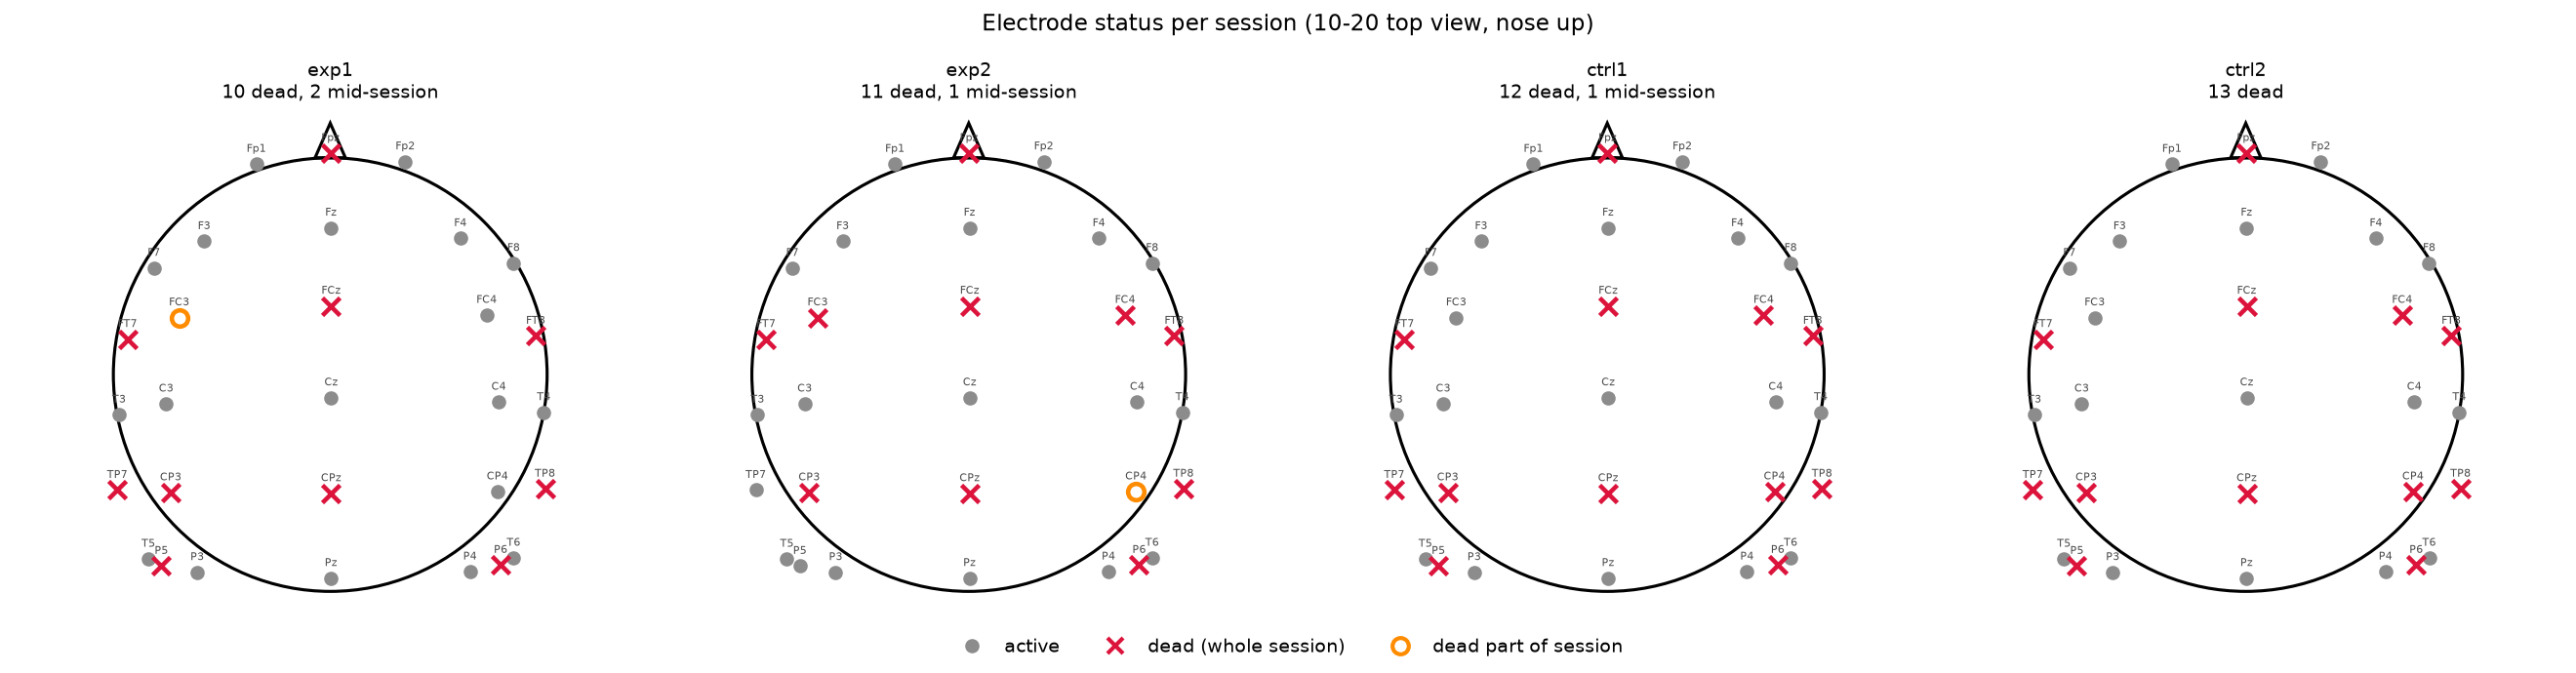
\includegraphics[width=\textwidth]{dead_topomaps.png}
\caption{Electrode status per session (10-20 top view). The same ring of electrodes (midline FCz/CPz,
lateral FT7/FT8, TP7/TP8, CP3, P5/P6, Fpz) is disconnected in every session and in both subjects;
orange marks channels that changed state mid-session (FC3 revived on day 1, CP4 died on day 2,
POz flapped in the control part 1).}
\label{fig:topo}
\end{figure}

\begin{figure}[ht]\centering
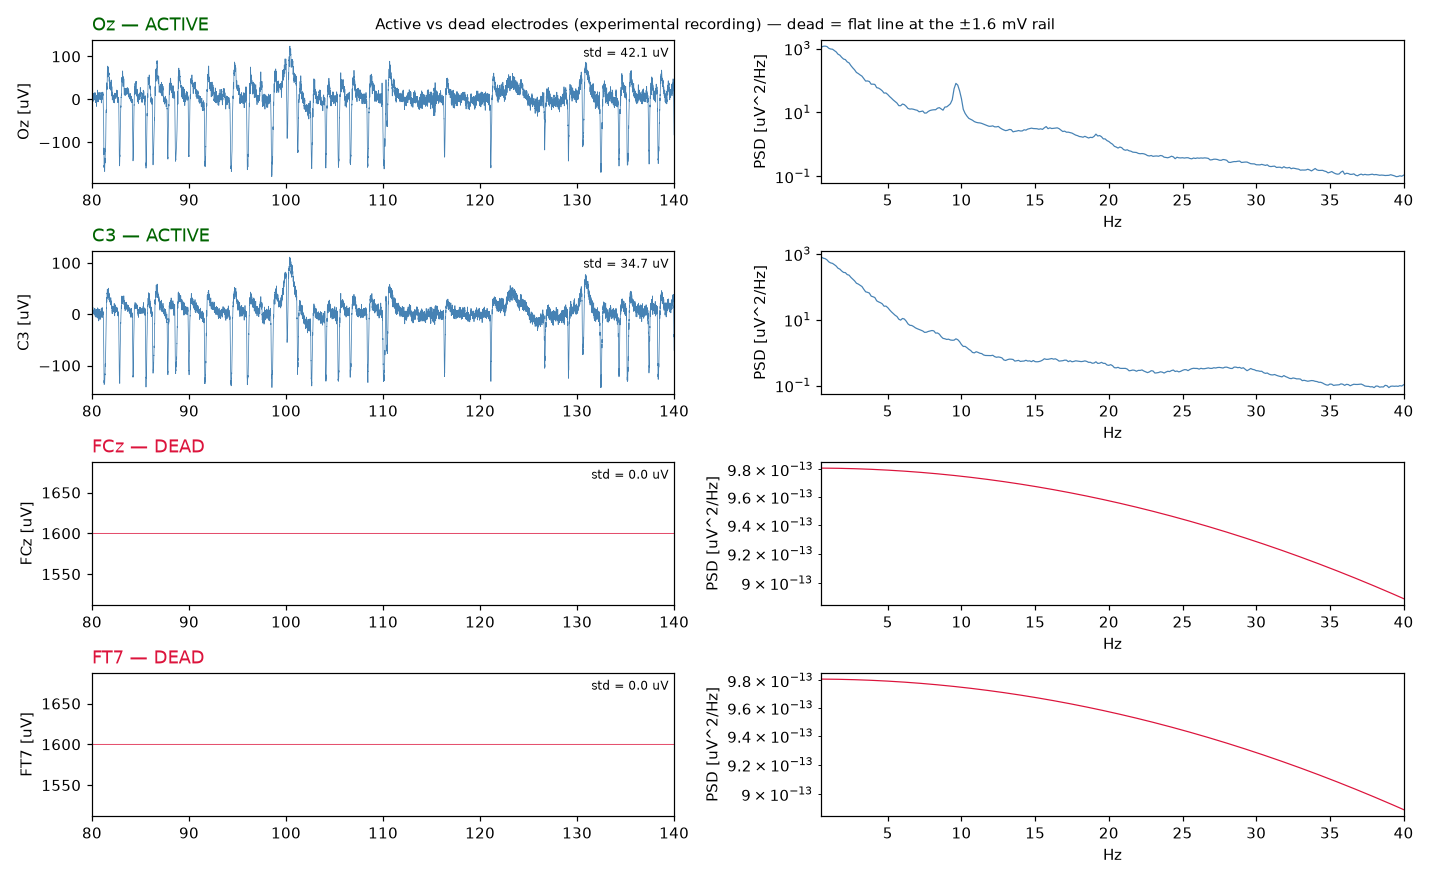
\includegraphics[width=0.95\textwidth]{dead_vs_active.png}
\caption{Active vs dead electrodes (the PWS participant, session 1). Active: real brain signal, 1/f spectrum, visible alpha
peak. Dead: flat line at the input rail, zero standard deviation, spectrum is numerical noise
(16 orders of magnitude weaker).}
\label{fig:dead}
\end{figure}

Mid-session changes (need time-aware bad-channel lists during analysis):
\begin{itemize}\setlength\itemsep{0pt}
\item PWS s1: FC3 \textbf{revived} at $\sim$1050\,s (during reading); POz dropped at 90\,s.
\item PWS s2: CP4 died at $\sim$1250\,s (during speech).
\item the control part 1: POz flapping (live 0--140\,s, dead 140--1380\,s).
\end{itemize}

\subsection*{2.2 Auxiliary channels}
\begin{itemize}\setlength\itemsep{1pt}
\item \textbf{Resp2 was not connected in the control session} (confirmed): its trace is pure noise in
both parts. The breathing belt (Pesp) is a genuine signal in both parts of the control.
\item \textbf{GSR of the control part 1 is real} --- same amplitude scale and phasic pattern as part 2
(Fig.~\ref{fig:aux}); only the shared crash spike at the end of part 1 made the channels look
correlated.
\item GSR of PWS session 2 is \textbf{very weak} ($\sim$10$\times$ below session 1) --- phasic responses are
visible but the sensor was poorly attached.
\item Pesp (1st breathing sensor) is dead in both PWS sessions.
\end{itemize}

\begin{figure}[ht]\centering
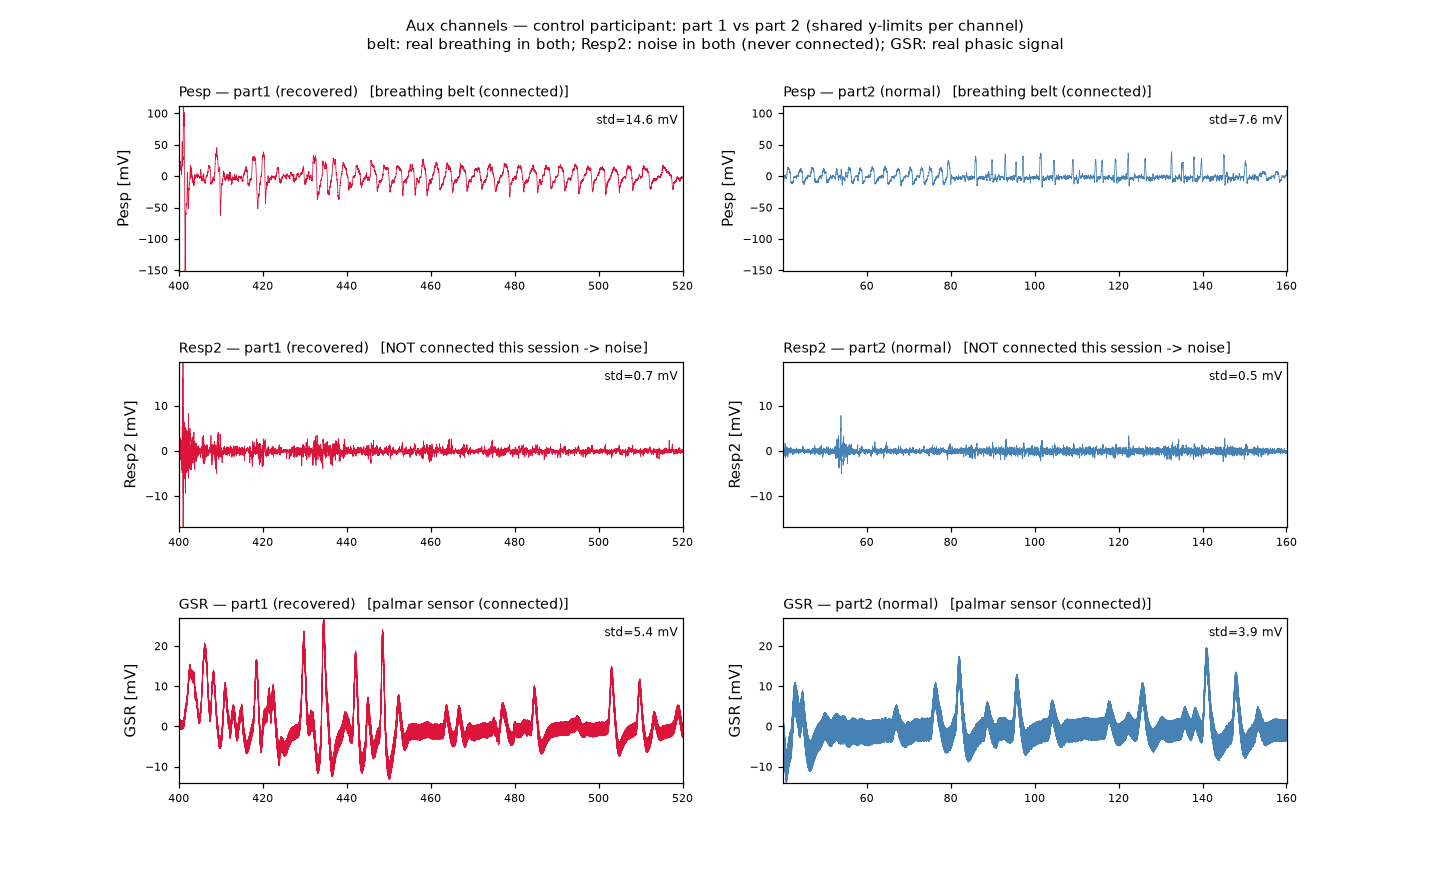
\includegraphics[width=0.95\textwidth]{aux_ctrl_parts.png}
\caption{Auxiliary channels of the control participant: part 1 (left) vs part 2 (right), shared scale per channel.
Breathing belt: real in both. Resp2: noise in both (never connected). GSR: real phasic signal in both.}
\label{fig:aux}
\end{figure}

\subsection*{2.3 Stage markers (events)}
\begin{itemize}\setlength\itemsep{1pt}
\item PWS s1: all 17 markers present; every fixed-duration stage is 180.0\,$\pm$\,0.1\,s --- the
marker timing is reliable (tens of ms).
\item PWS s2: one marker missing (\texttt{open\_raw3\_start}); the stage is reconstructed from the
179.98\,s gap between \texttt{reading\_finish} and \texttt{open\_raw3\_finish} --- exactly one rest block.
\item the control part 1: \textbf{no markers at all}. Root cause: the raw instrument file contains no event
block and no file footer --- markers are written when the recording closes normally, and the crash
prevented that. The conversion software is not at fault (it preserves markers in normal files).
Consequence: restarting the recording from the beginning after the crash would indeed have been the
right decision; stage boundaries for part 1 were estimated from the data itself (eyes-closed alpha
window and the breathing surge match the protocol order) and should be verified against the video.
\item ``100'' markers are redundant end-of-stage signals; all of them land within $\leq$1\,s after a
named stage end, with identical offsets across sessions --- they can serve as backup markers.
\end{itemize}

\section*{3. Does the data look as expected?}
\begin{itemize}\setlength\itemsep{2pt}
\item \textbf{Alpha rhythm at rest: yes, textbook.} Eyes-closed occipital alpha (8--12\,Hz) is
6--20$\times$ stronger than eyes-open in every recording; a clean 10\,Hz peak appears in the spectrum
only with eyes closed (Fig.~\ref{fig:psd}). Individual alpha frequency 9.6--9.9\,Hz, stable across
sessions.
\item \textbf{Motor artifacts during speech: yes.} High-frequency (30--80\,Hz) power is among the
highest of all stages in every recording; the recordings are artifact-rich overall (bad contacts move),
so artifact rejection must be relative/robust, not by absolute thresholds.
\item \textbf{Hyperventilation: half-confirmed.} Breathing \emph{depth} doubles-to-triples during
hyperventilation (belt amplitude), but \emph{rate} does not increase in any of the three recordings
(13--29/min both at rest and during hyperventilation). Either the subjects breathed deep-but-slow,
or the belt smooths out fast breathing. Worth checking the video.
\end{itemize}

\begin{figure}[ht]\centering
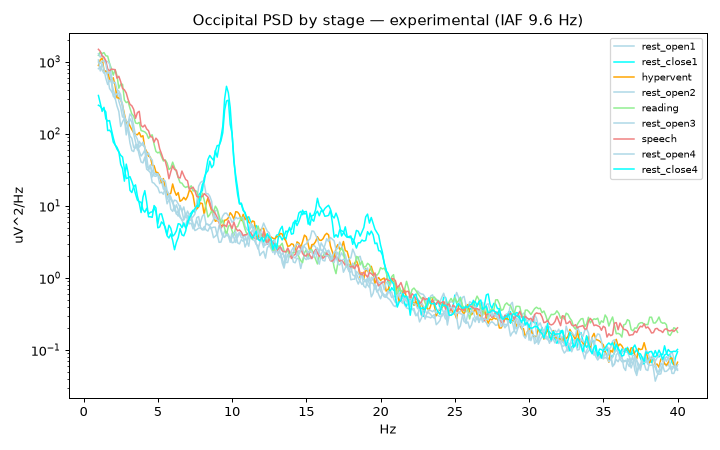
\includegraphics[width=0.49\textwidth]{psd_exp.png}\hfill
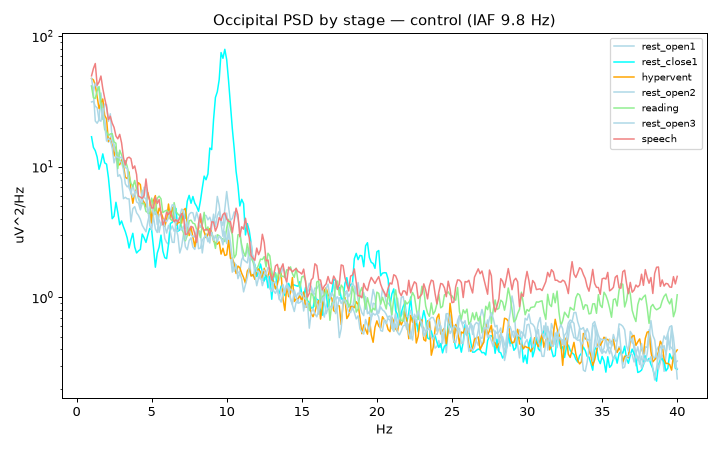
\includegraphics[width=0.49\textwidth]{psd_ctrl.png}
\caption{Occipital spectra by stage: eyes-closed curves (cyan) show a dominant 10\,Hz alpha peak in
both subjects; all other stages lack it.}
\label{fig:psd}
\end{figure}

\section*{4. Research-level findings}

\subsection*{4.1 Reaction to the hyperventilation challenge}
The canonical adult reaction: theta slow-wave ``build-up'' late in hyperventilation (only about a third
of healthy adults show it at all), clearing within 2 minutes after breathing normalizes.
\begin{center}\small
\begin{tabular}{@{}llllp{5.6cm}@{}}
\toprule
& theta during HV & late HV & 3 min after HV & verdict \\
\midrule
PWS, day 1 & $+69\%$ & $+98\%$ & still $+52\%$ & strong build-up, \textbf{delayed recovery} \\
\midrule
PWS, day 2 & $+2\%$ & $+6\%$ & $+19\%$ & \textbf{absent build-up} \\
\midrule
Control & $+29\%$ & $+33\%$ & $+30\%$ & mild, typical \\
\bottomrule
\end{tabular}
\end{center}
The \emph{same person} showed opposite reactions on the two days. The most likely explanation is
effort/compliance: breathing rate did not rise during hyperventilation in any recording, and the
day-2 response looks like half-hearted effort. The day-1 elevation of slow activity lasting more than
3 minutes is the only clinically-flavoured flag; physiologically, CO$_2$ recovers over $\sim$7 minutes,
so it may be benign. No high-amplitude rhythmic delta events (the clinically marked kind) occurred.
GSR jumped $+42\%$ during the challenge (PWS s1) --- strong sympathetic arousal.
After hyperventilation, eyes-open alpha is elevated in \emph{all three} recordings --- a genuine
post-challenge state or habituation; a second pre-challenge baseline would separate the two.

\begin{figure}[ht]\centering
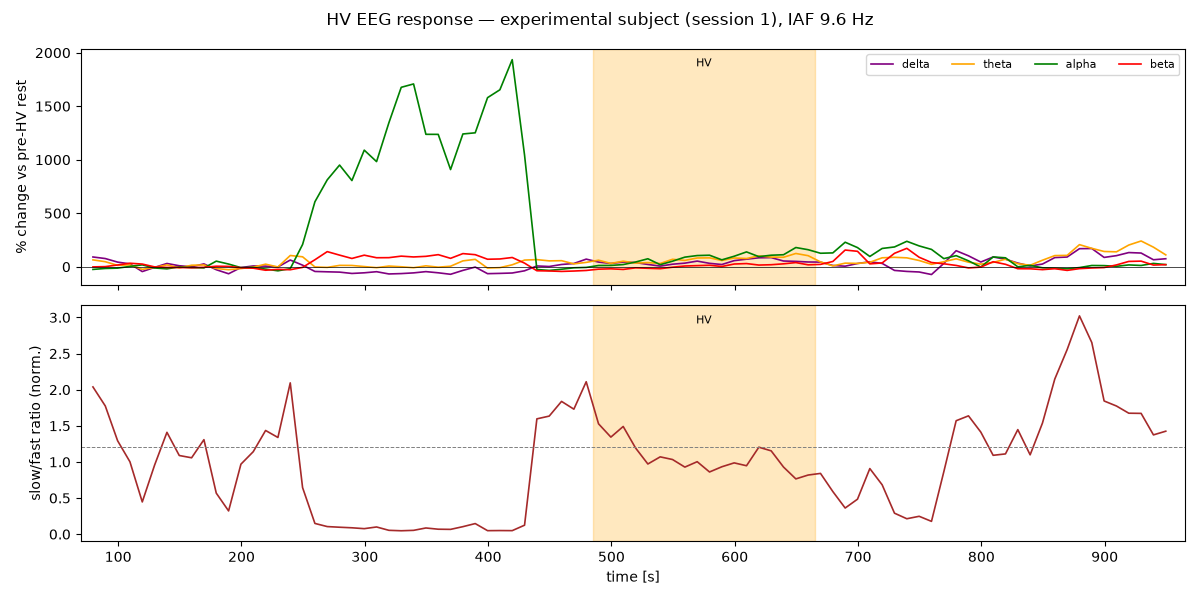
\includegraphics[width=0.9\textwidth]{hv_exp.png}
\caption{The PWS participant (session 1) around the hyperventilation block. Top: \% band-power
change vs the pre-challenge eyes-open rest; the large green alpha spike before the shaded
zone is the eyes-closed block. Bottom: slow/fast ratio stays elevated for minutes --- delayed recovery.}
\end{figure}

\subsection*{4.2 Speech: frontal ``effort'' theta separates the two people}
Frontal-midline theta (4--8\,Hz at Fz) is a classic marker of cognitive control and effortful
processing. During the narrative speech it rose by \textbf{+109\% and +69\% in the person with
stuttering (both sessions)} and by \textbf{--4\% in the control}. The same pattern appears during
reading aloud (+79\%/+53\% vs +6\%). This fits the stuttering literature's picture of elevated
speech-monitoring/effort load, and it replicated across days --- the most robust between-subject
difference found. Caveat: theta is blink-sensitive; the stuttering subject also blinks much more
(see below), so ICA-based cleaning is required before final numbers.

\subsection*{Listening vs answering inside the interview}
The interview stage contains both answering and listening to questions. Windows were classified
without a microphone by muscle (30--80\,Hz) activity: answering windows are the high-muscle bursts,
listening windows the quiet stretches between them (45--50\% of windows stayed ambiguous and were
excluded). The result refines the picture above:
\begin{center}\small
\begin{tabular}{@{}llll@{}}
\toprule
& frontal theta: listening vs rest & answering vs listening & blinks (listen $\to$ answer) \\
\midrule
PWS s1 & $+109\%$ & $+4\%$ & 59 $\to$ 59 /min \\
PWS s2 & $+71\%$ & $+1\%$ & 61 $\to$ 64 /min \\
Control & $-10\%$ & $+13\%$ & 16 $\to$ 28 /min \\
\bottomrule
\end{tabular}
\end{center}
In the stuttering subject the frontal-theta elevation is \emph{already maximal while listening} ---
it is an interview/engagement state, not articulatory effort per se. The control shows the opposite,
intuitive pattern: theta near baseline while listening and a modest $+13\%$ spike when actually
answering. Blinks in the stuttering subject stay high in both states; the control's blink rate
doubles when speaking. This is a single-subject observation with a crude listening/speaking proxy
(the interviewer's voice is also heard during ``listening'' windows), but it changes the headline:
the marker distinguishes \emph{being in dialogue}, not \emph{speaking}.

\subsection*{Language areas (Broca / Wernicke homologues)}
With 10-20 scalp electrodes these regions can only be approximated: Broca $\approx$ F7/F3 vs right
homologue F8/F4; Wernicke $\approx$ T3/T5 vs T4/T6. Comparing interview windows \emph{against rest}
is unreliable here: during the interview \emph{all} bands (alpha included) rise in amplitude ---
probably sweat lowering electrode impedance --- so absolute band changes are not interpretable.
The left/right asymmetry \emph{within} the same state is robust to that confound, and it is
informative (alpha power reflects relative cortical idling; less alpha = more activation):
\begin{center}\small
\begin{tabular}{@{}lcccc@{}}
\toprule
alpha L$-$R asymmetry, \% & \multicolumn{2}{c}{Broca homologue} & \multicolumn{2}{c}{Wernicke homologue} \\
\cmidrule(r){2-3}\cmidrule(l){4-5}
& answer & listen & answer & listen \\
\midrule
PWS, day 1 & $+27$ & $+27$ & $-15$ & $-15$ \\
PWS, day 2 & $+10$ & $+9$ & $-16$ & $-15$ \\
Control & $-4$ & $+2$ & $+19$ & $+1$ \\
Control (resumed) & $+2$ & $+2$ & $+9$ & $+9$ \\
\bottomrule
\end{tabular}
\end{center}
The stuttering subject shows a consistent pattern on both days: \textbf{left Broca homologue
relatively ``idling''} (positive = more left alpha = less left activation, $+10$ to $+27\%$) and
\textbf{right-dominant Wernicke homologue} ($-15\%$), i.e.\ a rightward lateralization bias during
language --- directionally matching the stuttering literature (left frontal/posterior-temporal
under-activation with right-hemisphere engagement). The control is balanced or left-leaning.
Two caveats: (1) the asymmetry is the same while answering and while listening --- again a tonic
language-mode state rather than a speech-evoked effect; (2) T3--T6 lie over the temporalis muscle,
so the Wernicke numbers are the weaker of the two. Final answers need fMRI-quality localization or
at least a high-density cap.

\subsection*{Reading aloud vs dialogue: same effort, different fluency}
The subject with stuttering was observed to be nearly fluent while conversing but noticeably
disfluent while reading aloud --- the opposite of the classic ``reading fluency effect'' reported in
the literature. Comparing the two vocal tasks directly (for the interview, only the speaking
windows, so both conditions are vocalizing) gives an informative negative result:
\begin{center}\small
\begin{tabular}{@{}lcccc@{}}
\toprule
& frontal theta & alpha & blinks & Broca L$-$R \\
\midrule
PWS s1: read $\to$ answer & $+3\%$ & $+10\%$ & 46$\to$60/min & $+19\to+27\%$ \\
PWS s2: read $\to$ answer & $+7\%$ & $+20\%$ & 46$\to$63/min & $0\to+10\%$ \\
Control: read $\to$ answer & $-1\%$ & (muscle-inflated) & 16$\to$23/min & $-4\to-4\%$ \\
\bottomrule
\end{tabular}
\end{center}
In the stuttering subject the cortical ``effort'' signature is essentially the \emph{same} in both
vocal tasks (frontal theta 14.1 vs 14.5 and 11.2 vs 12.0\,$\mu$V$^2$; GSR tonic level 278 vs 294\,mV,
SCR (skin conductance response) rate 13.8 vs 11.0/min) --- although fluency clearly differed. So the elevated theta does
\emph{not} track stuttering events; it marks the state of vocalizing under observation. The
reading-vs-dialogue fluency difference must live at the speech-motor planning level, which scalp EEG
with 36 channels cannot resolve --- and which no band-power contrast here captures. Disfluency
analysis proper requires audio (absent) plus video-annotated stuttering events time-locked to the
EEG: the one analysis we would most recommend adding to the protocol next time.

\subsection*{4.3 Arousal: blink rate and GSR}
\begin{itemize}\setlength\itemsep{1pt}
\item Blink rate at rest: \textbf{30--52/min in the stuttering subject vs 4--16/min in the control}
(2--4$\times$); rises by $\sim$35\% during speech in both. Consistent with elevated tonic
arousal/anxiety; valid as within-subject comparison.
\item Tonic GSR in PWS s1 climbs across the whole session (187 $\rightarrow$ 294\,mV from first rest
to speech) and decays only partially after speech --- arousal accumulates across the protocol.
\end{itemize}

\subsection*{4.4 Post-speech ``hypoxia-like'' effects: none}
The 3-minute rest after speech shows no slowing and no alpha decrease relative to pre-speech rest
(changes $\leq$1\%) in any recording. Speech-induced effects here are arousal and effort, and they
dissolve within minutes. (The hypoxia-like EEG signature belongs to hyperventilation via CO$_2$
drop, not to speaking.)

\subsection*{4.5 Other EEG anomalies --- screening results}
\begin{itemize}\setlength\itemsep{1pt}
\item \textbf{No epileptiform-like activity.} An automatic spike/sharp-wave screen plus visual review
of the top candidates found only blink artifacts (frontal slow deflections) and muscle bursts
(Fig.~\ref{fig:spikes}).
\item \textbf{No focal rhythmic delta episodes} anywhere.
\item \textbf{No 50\,Hz line noise}; no DC/saturation problems beyond the known dead electrodes.
\item \textbf{One flag:} in the stuttering subject, eyes-closed posterior alpha is markedly
right-dominant (parietal P3/P4 ratio $-54$ to $-68\%$, occipital $-23$ to $-35\%$), and the pattern
\emph{repeats on both days}; the control shows small unstable asymmetries. Could be physiological
(alpha asymmetry) or an electrode-contact artifact --- check impedance of P3/P4/O1/O2 before
interpreting.
\end{itemize}

\begin{figure}[ht]\centering
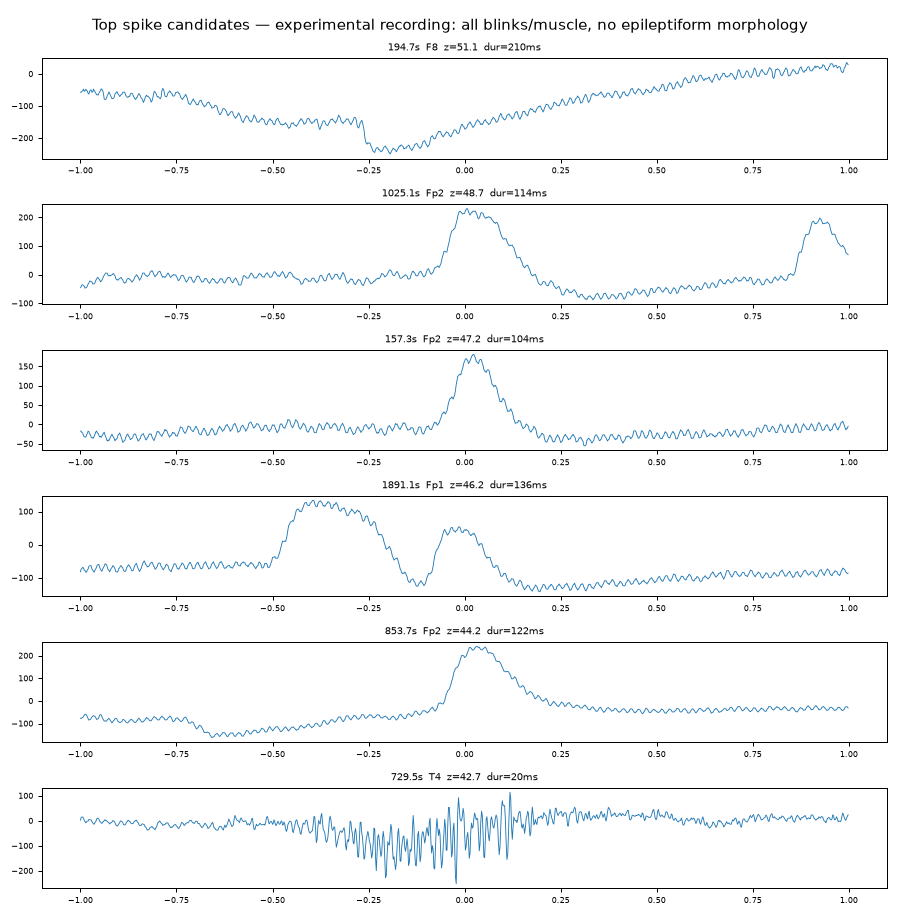
\includegraphics[width=0.9\textwidth]{spike_candidates.png}
\caption{Top automatic ``spike'' candidates (PWS session 1): all are blinks (Fp1/Fp2, slow positive
deflections) or muscle bursts (T4) --- no epileptiform morphology.}
\label{fig:spikes}
\end{figure}

\section*{5. Conclusions and recommendations}
\begin{enumerate}\setlength\itemsep{1pt}
\item All four recordings are usable for analysis: PWS s1 fully; PWS s2 with a weak GSR and one
reconstructed stage; the control part 1 with estimated stage boundaries (verify vs video) and without
Resp2; part 2 fully.
\item Hardware: the dead-electrode ring is identical across sessions and subjects $\rightarrow$
inspect electrodes/connector slots; find out why the impedance check passes with $\sim$1/3 of
electrodes disconnected.
\item Protocol: verify hyperventilation compliance (video; ideally EtCO$_2$); add a second
pre-challenge baseline; always restart recording after a crash (part 1 markers are unrecoverable).
\item Analysis: time-aware bad-channel lists; robust relative artifact rejection; ICA/CleanLine
before quantifying frontal theta and blink metrics.
\item Research leads worth pursuing with more subjects: sustained frontal-theta elevation across the
whole interview (present equally while listening and answering) in the stuttering subject,
replicated across days, versus a speaking-specific theta spike in the control; elevated resting
blink rate; delayed
post-hyperventilation recovery; right-dominant posterior alpha asymmetry (after ruling out contacts).
\end{enumerate}

\end{document}
